Because of the similarity of our task to with image encoding, we decided to take inspiration for our model architecture
from many different networks used for images segmentation. Our main inspiration was U-net \cite{Unet}.
This network exploits an autoencorder-like architecture to obtain the segmented image.
In particular, it uses convolution to extract features and maxpooling to downsample the image.
Another U-net element that inspired us is the use of concatenation in order to provide
residual connections between the "down" and "up" convolutions of the image. It must be noted that
the authors of the paper used cropping in order to perform these operations, as the feature dimensions between layers do not exactly match. 
It will be shown later that our architecture does not suffer from this issue since we decided to simply 
this process by having hidden states of equal size.
Another model architecture we took inspiration from was VoxSegNet \cite{VoxSegNet}. This architecture performs 
sequential extraction of features that are combined toghether, across different levels of extraction, to obtain a prediction. 
This is analogous to the residual, however with some more complexity added that won't be
discuss more in depth in this paper. 
The specific VoxSegNet element we imported in our model architecture is the use of convolutional layers with different dilation rates 
(atrous convolutions) in order to obtain features through kernels with larger fields of view.

Figure [\ref{fig:model}] represents the complete scheme of our model architecture.
\begin{figure*}[ht]
    \centering
    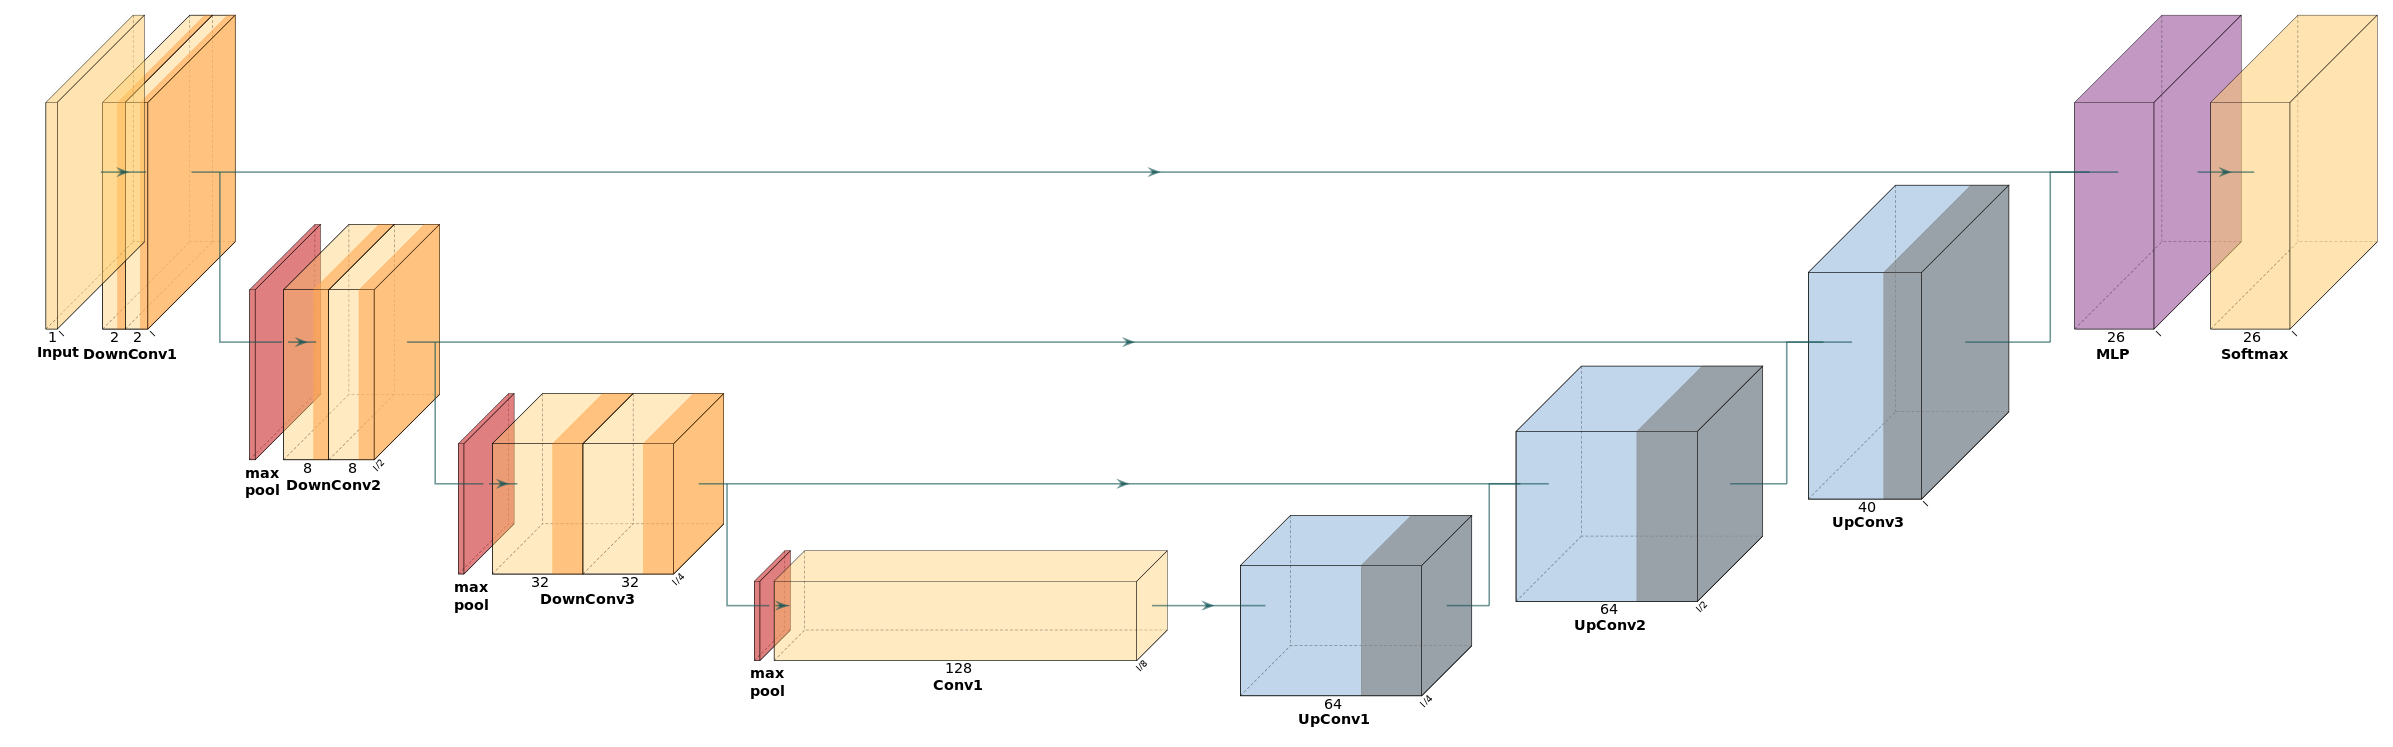
\includegraphics[width=\textwidth]{images/VUE_net_model.png}
    \caption{VUE-net architecture}
    \label{fig:model}
  \end{figure*}
